\newpage
\subsection{Simulation}\label{kap:simulation}
Sobald ein möglicher Lösungskandidat anhand der in Abschnitt \ref{sec:kandidatensuche} beschriebenen Suche gefunden
und dessen Initialgeschwindigkeit nach Abschnitt \ref{sec:initialgeschwindigkeit} berechnet wurde,
wird eine Simulation durchgeführt, um die Lösung definitiv zu bestätigen.
Durch das Anwenden verschiedener Anfangsgeschwindigkeiten der weissen Kugel können in diesem Schritt mehrere Situationen evaluiert werden.

Es wurde keine bestehende Physik-Engine für die Entwicklung der Simulation verwendet,
um maximale Flexibilität und Kontrolle über das Verhalten der Simulation zu haben.

Die Simulation wird durch die Definition eines physikalischen Systems wie in Kapitel \ref{kap:physikalisches_system} durchgeführt.
Hierbei gelten die Zuordnungen wie sie nachfolgend beschrieben werden.\\
\textbf{Ereignisse}
\begin{description}
    \item[Energy-Input-Node] Wird modelliert über die Eingabe der Energie der weissen Kugel. Ein spezifischer Node zur
    Modellierung wird nicht implementiert, es wird der Energy-Transfer-Node verwendet, wobei nur der Output-Wert relevant ist.
    \item[Energy-Transfer-Node] Tritt bei der Kollision zwischen zwei Kugeln oder einer Kugel mit der Bande auf.
    \item[No-Energy-Node] Tritt auf, wenn eine Kugel vom dynamischen in den statischen Zustand wechselt (ausrollt). In jedem
    Layer, wo eine Kugel statisch ist, wird sie durch diesen Node modelliert.
    \item[Out-of-System-Node] Sobald eine Kugel mit dem Zielkreis kollidiert, tritt dieses Ereignis auf. Dem System wird die
    Energie entzogen und die Kugel ist nicht mehr verfügbar.
\end{description}

\textbf{Kantenfunktion}
Die Kantenfunktion zwischen den Übergängen innerhalb des Layers bildet der Reibungsverlust der
Kugel über eine bestimmte Zeit oder einen bestimmten Ort.

\textbf{Dynamische/Statische Objekte}
Im Billiard gibt es nur die Kugeln als statische und/oder dynamische Objekte.

\textbf{Konstante Objekte}
Die konstanten Objekte bilden die Banden wie auch die Ziele.

Es wird ungefähr der Pseudoalgorithmus wie in \ref{alg:physikalisches_system} angewendet, optimal auf das Problem \glqq{}Billiard\grqq{}
abgestimmt. Es folgen die physikalischen Berechnungen zur Durchführung der Simulation.


\subsubsection{Reibungsverlust über die Zeit}
Die Geschwindigkeit einer Kugel wird durch die Reibung über die Zeit reduziert. Dazu wird die Formel der gleichförmig
beschleunigten Bewegung verwendet, wobei $\vec{v_0}$, $\vec{a}$ sowie $t$ gegeben sind.
\begin{align}
    \vec{v} = \vec{a} \cdot t + \vec{v_0}
\end{align}

\newpage
\subsubsection{Elastischer Stoss zweier Kugeln}\label{kap:simulation:elastischer_stoss_zweier_kugeln}
Die Kollision zweier Kugeln wird im Folgenden als zweidimensionaler elastischer Stoss \cite{wiki.elastischer_stoss_physik:1} angesehen.
Dabei ist es wichtig, zwei Komponenten beim Zusammenprall zu betrachten.
Dies ist einerseits das Liniensegment $\vec{s_z}$ zwischen den Mittelpunkten
der Kugeln sowie die orthogonal dazu stehende Gerade $\vec{s_t}$.
In Abbildung \ref{fig:Elastischer Stoss zweier Kugeln} ist ein elastischer Stoss dargestellt.

Die erste Kugel liegt zum Zeitpunkt der Kollision an der Position $Z_1$ und hat die Geschwindigkeit $\vec{v_1}$.
Die zweite Kugel liegt zum Kollisionszeitpunkt an der Position $Z_2$ und hat die Geschwindigkeit $\vec{v_2}$.
Ein Anteil der Geschwindigkeit von Kugel eins bei $Z_1$ wird der Kugel zwei in Richtung von $\vec{s_z}$ übergeben.
Die übrig gebliebene Energie zeigt in Richtung von $\vec{s_t}$.
Dasselbe gilt für die Kugel zwei.
Sie übergibt einen Teil ihrer Geschwindigkeit an Kugel eins ebenfalls in Richtung von $\vec{s_z}$.
Die verbleibende Energie der Kugeln zeigt jeweils in Richtung von $\vec{s_t}$.

\begin{figure}[h!]
    \begin{center}
        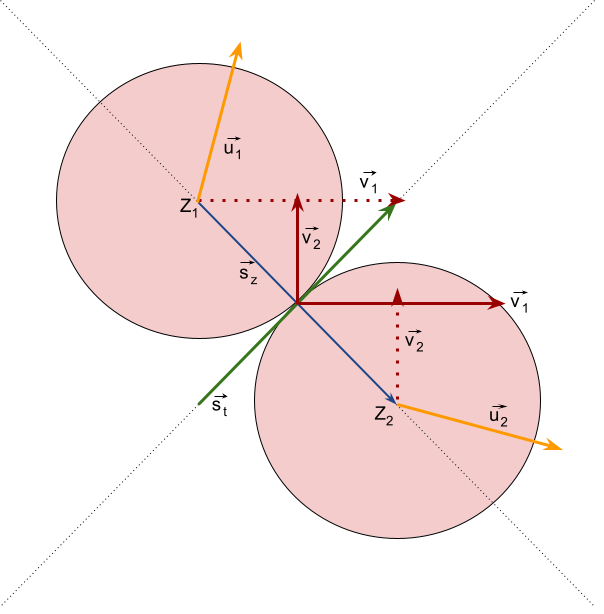
\includegraphics[width=0.4\linewidth]{../common/03_billiard_ai/resources/23_elastischer_stoss.png}
    \end{center}
    \caption{Elastischer Stoss zweier Kugeln:
    Die Geschwindigkeiten $\vec{v_1}$ und $\vec{v_2}$ der Kugeln werden auf die Richtungen $\vec{s_t}$ und $\vec{s_z}$ aufgeteilt und ausgetauscht.
    Resultierend rollen die Kugeln nach der Kollision mit den Geschwindigkeiten $\vec{u_1}$ und $\vec{u_2}$ weiter.
    }
    \label{fig:Elastischer Stoss zweier Kugeln}
\end{figure}

Die initialen Geschwindigkeiten $\vec{v^i_1}$ und $\vec{v^i_2}$ werden aufgrund eines Energieverlusts um eine
Konstante $E_v$, welche in Prozent angegeben wird, reduziert. Dies ist notwendig, da in der Realität durch Reibung
die Energie nicht vollständig weitergegeben wird.
\begin{align}
    \vec{v_1} = \vec{v^i_1} \cdot (1 - E_v)\\
    \vec{v_2} = \vec{v^i_2} \cdot (1 - E_v)\\
\end{align}
Um nun die neuen Geschwindigkeiten $\vec{u_1}$ und $\vec{u_2}$ zu berechnen, müssen die initialen Geschwindigkeiten
$\vec{v_1}$ sowie $\vec{v_2}$ auf die Komponenten in Richtung von $\vec{s_z}$ und $\vec{s_t}$ aufgeteilt werden.
\begin{align}
    \vec{z} = \vec{Z_2} - \vec{Z_1}\\
    \vec{z} = \vec{s_z}\\
    \hat{z} = \frac{\vec{z}}{\norm{\vec{z}}}
\end{align}
Von Interesse ist dabei nur $\hat{z}$.
Mit diesem Vektor kann die Komponente in Richtung $\vec{s_z}$ beider Geschwindigkeiten ermittelt werden.
\begin{align}
    \vec{v_{1,z}} = (\vec{v_1} \cdot \hat{z}) \cdot \hat{z}\\
    \vec{v_{2,z}} = (\vec{v_2} \cdot \hat{z}) \cdot \hat{z}
\end{align}
Mittels dieses neuen Vektors in Richtung $\vec{s_z}$ kann der Vektor in Richtung $\vec{s_t}$ berechnet werden.
\begin{align}
    \vec{v} = \vec{v_t} + \vec{v_z}\\
    \vec{v_t} = \vec{v} - \vec{v_z}
\end{align}
Daraus folgt für die jeweiligen Kugeln:
\begin{align}
    \vec{v_{1,t}} = \vec{v_1} - \vec{v_{1,z}}\\
    \vec{v_{2,t}} = \vec{v_2} - \vec{v_{2,z}}
\end{align}
Die neuen Geschwindigkeitsvektoren setzen sich wie beschrieben aus den jeweiligen Komponenten zusammen.
Das Resultat lautet wie folgt:
\begin{align}
    \vec{u_1} = \vec{v_{2,z}} + \vec{v_{1,t}}\\
    \vec{u_2} = \vec{v_{1,z}} + \vec{v_{2,t}}
\end{align}

\paragraph{Behandlung Rollverhalten} \hfill \\
Da eine Kugel nicht nur gleitet, sondern auch rollt und kaum Reibung mit der kollidierenden Kugel hat, hat dieses Rollen im
Falle einer Kugelkollision einen Einfluss auf den weiteren Verlauf der vorher dynamischen Kugeln.
Es werden zwei Ansätze erläutert. Die erste Variante behandelt das Rollen als ablenkende Kraft in eingehender Richtung mit konstantem Betrag.
Die zweite Variante berücksichtigt zusätzlich die Variabilität der Rollgeschwindigkeit. In Abbildung \ref{fig:einfluss_rollen} wird der Einfluss des
Rollens bei grossen wie auch kleinen Geschwindigkeiten erläutert.

Bei Variante eins wird der Einfluss des Rollens berücksichtigt,
indem bei den vorher dynamischen Kugeln ein Vektor mit konstantem
Betrag in der einkommenden Geschwindigkeitsrichtung auf den durch die elastische Kollision berechneten Vektor
$\vec{v_{k,t}}$ aufaddiert wird. Demnach gilt für den neuen Vektor $\vec{v_{k,t,n}}$ der Kugeln, wobei $A$ für die konstante Geschwindigkeit und
$\hat{v_k}$ für den normierten Vektor $\vec{v_k}$ der Kugel $k$ steht.
\begin{align}
    \vec{v_{1,t,n}} = \vec{v_{1,t}} + A \cdot \hat{v_1}\\
    \vec{v_{2,t,n}} = \vec{v_{2,t}} + A \cdot \hat{v_2}
\end{align}

Dieser Vektor $\vec{v_{k,t,n}}$ wird nun anstelle von $\vec{v_{k,t}}$ verwendet, wobei die maximale Energie des Vektors
auf die Eingangsenergie beschränkt wird.
\begin{align}
    \vec{u_1} = \vec{v_{2,z}} + \min{(\vec{v_{1,t,n}}, \norm{\vec{v_1}} \cdot \hat{{v_{1,t,n}}})}\\
    \vec{u_2} = \vec{v_{1,z}} + \min{(\vec{v_{2,t,n}}, \norm{\vec{v_2}} \cdot \hat{v_{2,t,n}})}
\end{align}

\begin{figure}[h!]
    \centering
    \begin{subfigure}[b]{0.6\textwidth}
        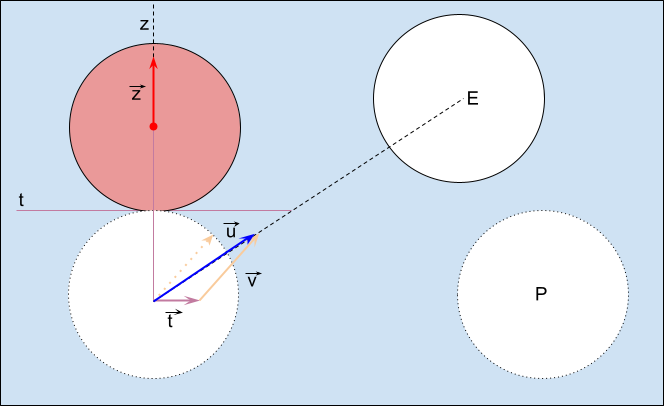
\includegraphics[width=1\textwidth]{../common/03_billiard_ai/resources/33_rollen_kleine_geschwindigkeit.png}
        \caption{Rolleinfluss bei kleiner Geschwindigkeit}
        \label{fig:rollen_kleine_geschwindigkeit}
    \end{subfigure}\\
    \begin{subfigure}[b]{0.6\textwidth}
        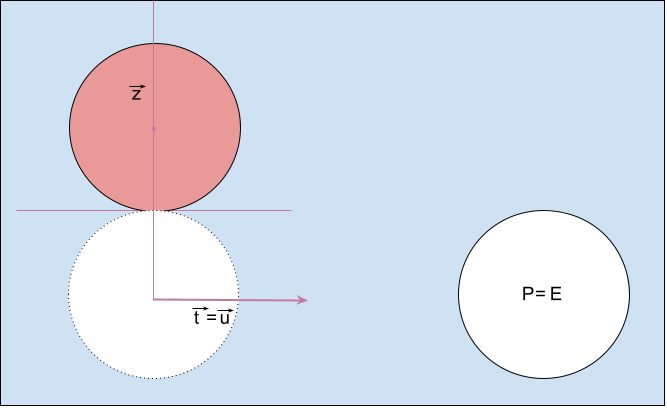
\includegraphics[width=1\textwidth]{../common/03_billiard_ai/resources/34_gleiten_grosse_geschwindigkeit.png}
        \caption{Kein Rollen bei grosser Geschwindigkeit}
        \label{fig:gleiten_grosse_geschwindigkeit}
    \end{subfigure}
    \caption{(a) Eine einkommende Geschwindigkeit $\vec{v}$ wird auf die Komponenten $\vec{z}$ und $\vec{t}$ nach dem
    elastischen Stoss aus Kapitel \ref{kap:simulation:elastischer_stoss_zweier_kugeln} aufgeteilt.
    Ohne Berücksichtigung des Rollens wird die Position der weissen Kugel bei $P$ berechnet, die effektive Position ist bei $E$.
        (b) Bei grösserer Geschwindigkeit fängt die Kugel erst später an zu rollen. Zum Kollisionszeitpunkt gleitet sie
        in diesem Fall nur und es gilt der zweidimensionale elastische Stoss wie in
        Kapitel \ref{kap:simulation:elastischer_stoss_zweier_kugeln} beschrieben.
        $P$ und $E$ stimmen in diesem Fall überein.}
    \label{fig:einfluss_rollen}
\end{figure}

Variante zwei verfolgt einen ähnlichen Ansatz, jedoch wird bei der Berechnung von $\vec{v_{k,t,n}}$ anstelle des normierten
der initiale Geschwindigkeitsvektor verwendet, welcher mit einem Prozentsatz skaliert wird. Dadurch wird die Variabilität
berücksichtigt. Es gilt, dass $A$ zwischen $0$ und $1$ liegt.
\begin{align}
    \vec{v_{1,t,n}} = \vec{v_{1,t}} + A \cdot \vec{v_1}\\
    \vec{v_{2,t,n}} = \vec{v_{2,t}} + A \cdot \vec{v_2}
\end{align}

Die Berechnung von $\vec{u_1}$ sowie $\vec{u_2}$ geschieht auf dieselbe Art und Weise wie bei Variante eins.
Implementiert wurde die zweite Variante, da die variable Rollenergie dadurch mitberücksichtigt wird.

\newpage
\subsubsection{Bandenreflektion}
Sofern eine Kugel an eine Bande stösst, wird diese abgelenkt. In dem hier beschriebenen Modell wird der Drall \cite{wiki.spin:1},
welcher die Bahn einer Kugel nach Kollision mit der Bande ablenken würde, ignoriert.
Das bedeutet, es wird davon ausgegangen, dass der Ausfallswinkel nach der Bandenreflektion gleich dem Einfallswinkel sei.
Dazu kann die folgende Formel \cite{paulbourke.reflected_ray:1} verwendet werden, wobei $I$ der einfallende
und $R$ der ausgehende Weg der Kugel und $N$ der Normalenvektor der Bande sind:
\begin{align}
    R = I - 2 \cdot N \cdot (I \cdot N)
\end{align}

Da bei einer Bandenkollision Energie verloren geht, wird dieses Verhalten mit der Konstanten $E_v$ modelliert.
Diese gibt den Verlust in Prozent an.
\begin{align}
    R = (I - 2 \cdot N \cdot (I \cdot N)) \cdot \frac{1}{1 + E_v}
\end{align}

\subsubsection{Kollisionsprüfung}\label{kap:simulation:kollisionspruefung}
Während der Simulation ist es notwendig zu prüfen, welche Kugeln mit welchen kollidieren könnten.
Um zu wissen, ob eine Kugel eine Strecke zurücklegen kann, ohne mit einer anderen Kugel zu kollidieren,
muss für jede andere Kugel geprüft werden, ob diese im Weg liegt.
Daher sollte dieser Test effizient sein.
Für den Test wird die zurückzulegende Strecke als Liniensegment zwischen Punkt $A$ und Punkt $B$ und die Position
einer zu testenden Kugel $C$ als Punkt verstanden. Anschliessend wird der Abstand zwischen dem Punkt $C$ und dem
Liniensegment $AB$ geprüft, ob dieser kleiner als der Kugeldurchmesser ist.
Sofern dies der Fall ist, liegt die Kugel an der Position $C$ im Weg und es würde eine Kollision stattfinden,
sofern die Ausgangskugel die Strecke $AB$ rollt.
Dies wird für jede Kugel geprüft.
In Abbildung \ref{fig:kollisionsprüfung} ist eine Situation dargestellt.

\begin{figure}[h!]
    \begin{center}
        \includegraphics[width=0.4\linewidth]{../common/03_billiard_ai/resources/kollisionsprüfung.png}
    \end{center}
    \caption{Damit eine Kugel von A nach B rollen kann, darf keine Kugel C auf dem Weg liegen,
        deren Abstand zum Liniensegment AB kleiner als der Kugeldurchmesser ist.
        In der abgebildeten Situation ist die Kugel C zu nahe und es würde eine Kollision stattfinden.
    }
    \label{fig:kollisionsprüfung}
\end{figure}

\subsubsection{Ereignis - Energie-Transfer über Kugelkollision}
Dieses Ereignis beschreibt die Kollision mit einer anderen Kugel zum Zeitpunkt $t$.
Bekannt sind dabei die Beschleunigung $\vec{a}$, die Geschwindigkeit $\vec{v}$ und der Ort $\vec{s}$ beider Kugeln.
Diese werden entsprechend indexiert.
Die Beschleunigung $\vec{a}$ ist durch die Herleitung in Kapitel \ref{anhang:herleitung:beschleunigung} gegeben.

Weiterhin sind folgende Abstraktionen bekannt:
\begin{align}
    \vec{\Delta a} = \vec{\Delta a}_1 - \vec{\Delta a}_2\\
    \vec{\Delta v} = \vec{\Delta v}_1 - \vec{\Delta v}_2\\
    \vec{\Delta s} = \vec{\Delta s}_1 - \vec{\Delta s}_2
\end{align}

Es entsteht ein Polynom vierten Grades (Herleitung in Anhang \ref{anhang:herleitung:event:dynamicObjectCollision}).
Um diese Gleichung zu lösen, bedarf es der entsprechenden Lösungsformel \cite{wiki.polynom:1}:
\begin{align}
    ax^4 + bx^3 + cx^2 + dx + e = 0\\
    x_{1,2} = -\frac{b}{4a} - S \pm \frac{1}{2}\sqrt{-4S^2 - 2p + \frac{q}{S}}\\
    x_{3,4} = -\frac{b}{4a} + S \pm \frac{1}{2}\sqrt{-4S^2 - 2p - \frac{q}{S}}\\
    p = \frac{8ac - 3b^2}{8a^2}\\
    q = \frac{b^3 - 4abc + 8a^{2}d}{8a^3}\\
    S = \frac{1}{2}\sqrt{-\frac{2}{3}p + \frac{1}{3a}(Q + \frac{\Delta_0}{Q})}\\
    Q = \sqrt[3]{\frac{\Delta_1 + \sqrt{\Delta_{1}^2 - 4\Delta_{0}^3}}{2}}\\
    \Delta_0 = c^2 - 3bd + 12ae\\
    \Delta_1 = 2c^3 - 9bcd + 27b^{2}e + 27ad^2 - 72ace
\end{align}

Wobei die Koeffizienten folgendermassen lauten:
\begin{align}
    a = \frac{1}{4} \cdot (\vec{\Delta a} \cdot \vec{\Delta a})\\
    b = \vec{\Delta a} \cdot \vec{\Delta v}\\
    c = \vec{\Delta a} \cdot \vec{\Delta s} + \vec{\Delta v} \cdot \vec{\Delta v}\\
    d = 2 \cdot (\vec{\Delta v} \cdot \vec{\Delta s})\\
    e = \vec{\Delta s} \cdot \vec{\Delta s} - D^2
\end{align}

Durch Lösen des Polynoms werden alle Zeitpunkte $x_{1-4} = t_{1-4}$ bestimmt, wobei der relevante Zeitpunkt $t$ der
Erste ist.
\begin{align}
    t = \min{(t_1, t_2, t_3, t_4)}
\end{align}

\paragraph{Performanceverbesserungen} \hfill \\
Das Lösen dieses Gleichungssystems erfordert viel Rechenzeit, was die Frage nach Performanceverbesserungen aufwirft.
Diese werden durch Vorbedingungen erzielt, welche geprüft werden. Es findet zu Beginn eine Fallunterscheidung statt.

Wenn die zweite Kugel statisch ist, so kann die Distanz dieser Kugel zur halben Geraden der Laufrichtung der ersten Kugel geprüft werden.
Die Laufrichtung der ersten Kugel kann mit deren Position $P_1$ und des Geschwindigkeitsvektors $\vec{v}$ als halbe Gerade $g$ definiert werden.
Sofern die Distanz $d$ zwischen der zweiten Kugel und dieser Geraden kleiner oder gleich dem Kugeldurchmesser ist,
dann liegt die zweite Kugel der ersten Kugel im Weg.
Nur dann könnte es zur Kollision kommen.
Sämtliche Angaben beziehen sich auf die Grafik \ref{fig:kugelkollision_vorbedingung_statisch}.

\begin{figure}[h!]
    \begin{center}
        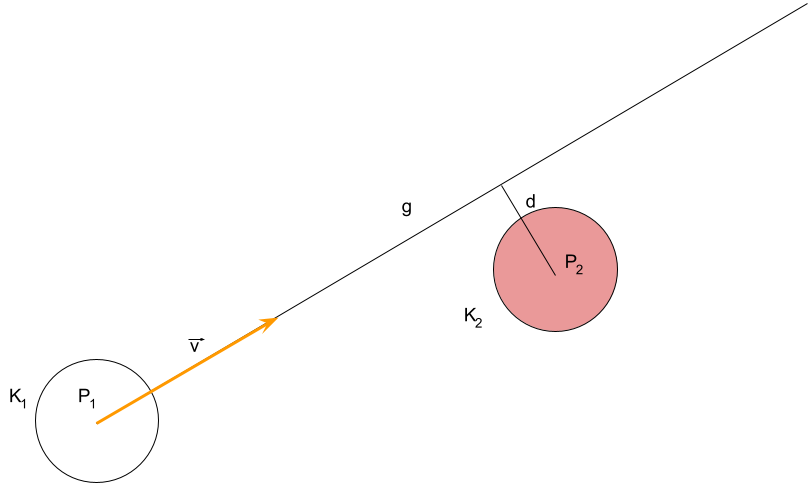
\includegraphics[width=0.4\linewidth]{../common/03_billiard_ai/resources/24_vorbedingung_kugelkollision_statisch.png}
    \end{center}
    \caption{Vorbedingung einer Prüfung auf Kollision zwischen Kugeln bei statischer Beteiligung.
    Die Kugel an Position $P_1$ ist dynamisch, die Kugel an Position $P_2$ ist statisch.}
    \label{fig:kugelkollision_vorbedingung_statisch}
\end{figure}

Sobald beide Kugeln dynamisch sind reicht eine einfache Prüfung auf die Distanz nicht mehr. Es muss ein Schnittpunkttest der beiden halben Geraden, definiert durch die
beiden Geschwindigkeitsvektoren, durchgeführt werden. Hierbei ist der Durchmesser der Kugel zu beachten, dies
wird in Abbildung \ref{fig:kugelkollision_vorbedingung_dynamisch} dargestellt.
\begin{figure}[h!]
    \begin{center}
        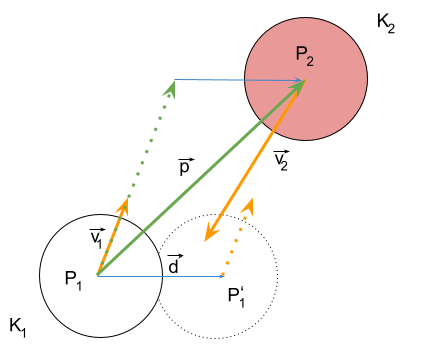
\includegraphics[width=0.4\linewidth]{../common/03_billiard_ai/resources/25_vorbedingung_kugelkollision_dynamisch.png}
    \end{center}
    \caption{Vorbedingung einer Prüfung auf Kollision zwischen dynamischen Kugeln.}
    \label{fig:kugelkollision_vorbedingung_dynamisch}
\end{figure}

Daher wird der Vektor $\vec{p}$ zwischen den Positionen $P_1$ und $P_2$ gebildet (grün).
\begin{align}
    \vec{p} = P_2 - P_1
\end{align}
Der erhaltene Vektor wird auf den Geschwindigkeitsvektor $\vec{v_1}$ projiziert (grün gestrichelt).
\begin{align}
    \vec{p'} = (\vec{p} \cdot \hat{v_1}) \cdot \hat{v_1}
\end{align}
Danach wird der Zwischenvektor $\vec{d}$ gebildet (blau).
\begin{align}
    \vec{d} = \vec{p} - \vec{p'}
\end{align}

Die Kugel $K_1$ wird um diesen Vektor verschoben, es resultiert $P^{'}_1$.
\begin{align}
    P^{'}_1 = P_1 + \vec{d}
\end{align}
Von dieser Position aus kann nun ein Schnittpunkttest zwischen den beiden
halben Geraden, durch die Geschwindigkeitsvektoren definiert, durchgeführt werden.

Zudem gibt es zwei Spezialfälle zu beachten. Der erste beschreibt die Handhabung bei paralleler Fortbewegung
der Kugeln. Da dies ein sehr seltener Fall ist und
wohl kaum auftreten wird, wird die Berechnung zugelassen, wenn der Vektor $\vec{d}$ kleiner oder gleich gross
wie der Durchmesser ist. Die Situation wird in Abbildung \ref{fig:kugelkollision_vorbedingung_dynamisch_parallel} erläutert, die Berechnungen für den Vektor $\vec{d}$
sind äquivalent zu den vorhergehenden Berechnungen.
\begin{figure}[h!]
    \begin{center}
        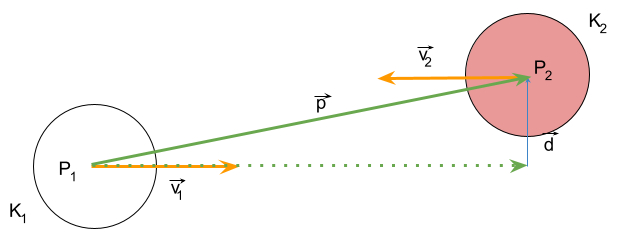
\includegraphics[width=0.4\linewidth]{../common/03_billiard_ai/resources/26_vorbedingung_kugelkollision_dynamisch_parallel.png}
    \end{center}
    \caption{Vorbedingung einer Prüfung auf Kollision zwischen dynamischen parallellaufenden Kugeln}
    \label{fig:kugelkollision_vorbedingung_dynamisch_parallel}
\end{figure}

Der letzte Spezialfall befasst sich mit der Tatsache, dass ein Schnittpunkttest, so wie er unter Berücksichtigung der
obigen Fälle durchgeführt wird, kein Ergebnis findet, wenn der Schnittpunkt hinter einer der Geraden liegt.
Diese Situation kann in Abbildung \ref{fig:kugelkollision_vorbedingung_dynamisch_hintereinander} entnommen werden.
Es ist ersichtlich, dass der Geschwindigkeitsvektor $\vec{v_1}$ einen grösseren Betrag aufweist als der
Geschwindigkeitsvektor $\vec{v_2}$. Um diesem Umstand Rechnung zu tragen, wird die Startposition der Geraden um den
Durchmesser nach hinten verschoben.
\begin{figure}[h!]
    \begin{center}
        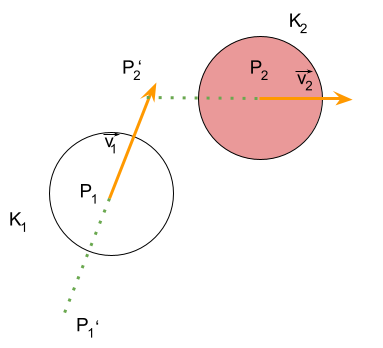
\includegraphics[width=0.4\linewidth]{../common/03_billiard_ai/resources/27_vorbedingung_kugelkollision_dynamisch_hintereinander.png}
    \end{center}
    \caption{Vorbedingung einer Prüfung auf Kollision zwischen dynamischen hintereinander verlaufenden Kugeln}
    \label{fig:kugelkollision_vorbedingung_dynamisch_hintereinander}
\end{figure}

\subsubsection{Ereignis - Energie-Transfer über Bandenkollision}
Dieses Event beschreibt die Kollision mit der Bande. Es soll der Zeitpunkt $t$ der Kollision mit der Bande festgestellt werden.
Der Algorithmus funktioniert so, dass zuerst geprüft wird, ob eine Kollision stattfinden kann.
Dies erfolgt über einen Schnittpunkt-Test zwischen einer Linie und einem Liniensegment.
Eine Bande kann als Liniensegment zwischen dem Startpunkt $R_1$ und $R_2$ betrachtet werden. Diese Punkte müssen demnach bekannt sein.
Weiterhin ist der Geschwindigkeitsvektor $\vec{v}$ und die Position der Kugel $C$ bekannt.
Aufgrund dieser Informationen kann eine Linie definiert werden.

Die Punkte $R_1$ und $R_2$ werden um den Kugelradius zur Tischmitte verschoben,
damit dem Kugelradius Rechnung getragen wird und dieser nicht weiter betrachtet werden muss.
Daraus ergeben sich $R_1'$ und $R_{2'}$ (Herleitung in Anhang \ref{anhang:herleitung:event:collisionWithRail}).

Erster Schritt - Prüfe, ob Kollision möglich:\\
Dazu wird festgestellt, ob ein Schnittpunkt zwischen der Lauflinie der Kugel und dem Liniensegment der
Bande existiert, siehe Anhang \ref{anhang:herleitung:event:collisionWithRail}.
Sofern kein Schnittpunkt vorliegt, können weitere Tests abgebrochen werden, da keine Kollision mit der Bande stattfinden wird.

Zweiter Schritt - Ort der Kollision bestimmen:\\
Betrachte dazu eine der Gleichungen mit zugehörigem $\lambda$:
\begin{align}
    \vec{s(\lambda_1)} = \vec{R_1'} + \lambda_1 \cdot \vec{\Delta R'}\\
    \vec{s(\lambda_2)} = \vec{C} + \lambda_2 \cdot \vec{v}
\end{align}

Dritter Schritt - Zeitpunkt der Kollision bestimmen:\\
Dies kann über die folgenden Gleichungen gelöst werden:
\begin{align}
    \Delta t_1 = \frac{-v + \sqrt{v^2 + 2 \cdot a \cdot \Delta s}}{a}\\
    \Delta t_2 = \frac{-v - \sqrt{v^2 + 2 \cdot a \cdot \Delta s}}{a}
\end{align}
Bevor die Lösung zu $t_1$ und $t_2$ berechnet wird, muss jedoch der Radikand auf folgende Eigenschaft geprüft werden:
\begin{align}
    0 \leq v^2 + 2 \cdot a \cdot \Delta s
\end{align}
Nur in diesem Fall gibt es eine Lösung und somit an dieser Position eine Kollision. Ansonsten hat die Kugel vorher schon
ihre Gesamtenergie verloren und steht still. Es wird das Minimum der beiden Zeiten $\Delta t_1$ und $\Delta t_2$ verwendet.

Probleme hat dieser Ansatz ergeben, wenn die Kugel z.B. nahe der Bande rollt oder teilweise auch aufgrund der Ungenauigkeiten
beim Rechnen mit Fliesskommazahlen. So wurde die Kollision mit derselben Bande mehrfach aufeinanderfolgend detektiert und
die Kugel konnte so durch die Bande hindurchrollen. Das Problem wurde behoben, indem
die letzte Bande, mit welcher die Kugel kollidierte, von der Ereignisberechnung ausgeschlossen wurde. Die Bande wird
erst wieder miteinbezogen, wenn die Kugel eine andere Bande oder eine andere Kugel getroffen hat.

\subsubsection{Ereignis - Totaler Energieverlust}
Dieses Ereignis trifft ein, sobald eine Kugel stillsteht.
Der Zeitpunkt wird über die Formel \ref{eq:ereignis:out_of_energy:00} beschrieben (Herleitung in Anhang \ref{anhang:herleitung:event:outOfEnergy}).
Die Beschleunigung $\vec{a}$ ist durch die Herleitung in Kapitel \ref{anhang:herleitung:beschleunigung} gegeben.

\begin{align}
    t = \max{(\frac{-v_{0,x}}{a_x}, \frac{-v_{0,y}}{a_y})}\label{eq:ereignis:out_of_energy:00}
\end{align}

\subsubsection{Ereignis - Verlassen des Systems}
Der Ereigniszeitpunkt erfolgt über zwei Schritte. Im ersten Schritt wird der Kollisionspunkt der Kugel mit dem
Zielkreis bestimmt. Anhand dieser Information kann die zurückgelegte Distanz der Kugel bestimmt werden.
Es gelten die folgenden Definitionen:\\
$\vec{C} = $ Zielmittelpunkt\\
$\vec{p} = $ Position der Kugel\\
$\hat{v} = $ Normierte Geschwindigkeit der Kugel\\

Die nachfolgende Formel definiert, mit welchem Faktor der Geschwindigkeitsvektor multipliziert werden muss, damit
er die Länge der zurückzulegenden Distanz zum Kollisionsort mit dem Ziel erreicht (Herleitung in Anhang \ref{anhang:herleitung:event:targetCollision}).
Zu beachten ist, dass $l$ nur gültig ist, wenn es grösser als $0$ ist.
\begin{align}
    l_1 = \frac{-(2 \cdot \hat{v} \cdot (\vec{p} - \vec{C})) + \sqrt{4 \cdot (\vec{p} - \vec{C}) \cdot (\vec{p} - \vec{C}) \cdot r^2}}{2}\\
    l_2 = \frac{-(2 \cdot \hat{v} \cdot (\vec{p} - \vec{C})) - \sqrt{4 \cdot (\vec{p} - \vec{C}) \cdot (\vec{p} - \vec{C}) \cdot r^2}}{2}\\
    l = \max{(\min{(l_1, l_2)}, 0)}\\
    \vec{d(l)} = l \cdot \hat{v}
\end{align}

Nachdem die Distanz bestimmt wurde, kann der Kollisionszeitpunkt berechnet werden (Herleitung in Anhang \ref{anhang:herleitung:event:targetCollision}).
Die Beschleunigung $\vec{a}$ ist durch die Herleitung in Kapitel \ref{anhang:herleitung:beschleunigung} gegeben.
Zu beachten ist, dass keine Lösung existiert, wenn die Diskriminante kleiner denn $0$ ist. Die Kugel rollt zu langsam und
der Reibungsverlust ist zu gross, als dass sie den Zielkreis erreichen könnte.
\begin{align}
    t_1 = \frac{-\norm{\vec{v}} + \sqrt{\norm{\vec{v}}^2 + 2 \cdot \norm{\vec{a}} \norm{\vec{d(l)}}}}{\norm{\vec{a}}}\\
    t_2 = \frac{-\norm{\vec{v}} - \sqrt{\norm{\vec{v}}^2 + 2 \cdot \norm{\vec{a}} \norm{\vec{d(l)}}}}{\norm{\vec{a}}}\\
    t = \min{(t_1, t_2)}
\end{align}

\subsubsection{Ereignis - Rollen}
Wenn eine Kugel zentral angestossen wird, dann gleitet sie einen Moment, ohne zu rollen. Die Eigenschaft des
Rollens wird ebenso als Ereignis geführt.
Der Zeitpunkt, wann dieses Ereignis eintritt, kann über die Formel \ref{eq:rollzeitpunkt_2} berechnet werden,
wobei $\mu$ für den Gleitreibungskoeffizienten steht.
Die Herleitung erfolgt in Kapitel \ref{anhang:herleitung:event:rollen}.

\begin{align}
    t = \frac{v_0}{\frac{7}{2} \cdot g \cdot \mu}\label{eq:rollzeitpunkt_2}
\end{align}

Dieser Zeitpunkt wird einmal beim Anstossen einer Kugel berechnet und zwischengespeichert.
Würde dieses Ereignis nach jedem Vorherigen neu berechnet werden, so würde der Rollzeitpunkt immer weiter in der Zukunft liegen.
Dieses Zwischenspeichern wäre nicht nötig, würde die Simulation sämtliche Ereignisse vorausberechnen, zwischenspeichern,
abarbeiten und bei Bedarf invalidieren. Eine mögliche Verbesserung des Algorithmus wird in Kapitel \ref{anhang:simulation:algorithmus} beschrieben.

Weiterhin wird angenommen, dass gleitende Kugeln nach einer Kollision mit einer anderen Kugel weitergleiten. Es ist
auch bekannt, dass die Kugel nach der Kollision mit der Bande sofort zu rollen beginnt \cite{sciphysik:kugelohneschlupf}.

\subsubsection{Bewertungsfunktion}
Wie auch die Suche nach einem guten Lösungskandidaten muss das Endresultat der Simulation bewertet werden.
In dem Fall geht es um die Bestimmung der Belohnung eines Stosses oder umgekehrt die Bestrafung in Form von Kosten.
In einem ersten Schritt wird die Belohnung berechnet, welche sich an der Anzahl und dem Typen der eingelochten Kugeln richtet.
Es gibt die Schwarze (7), Pinke (6), Blaue (5), Braune (4), Grüne (3), Gelbe (2) und Rote (1) Kugel.
Die Punkte sind jeweils hinter dem Typen aufgeführt.
In einem Stoss wird eine maximal mögliche Punktzahl von $7$ definiert.
Sollten mehr Punkte erzielt werden, wird dies im Weiteren keinen Einfluss mehr haben, dazu später mehr.
Dieser Score $S$ wird durch eine Normierung der erzielten Punkte $p$ anhand der
maximal möglichen Punkte $p_{max}$ verkleinert. Zumeist wird er zwischen $0$ und $1$ liegen, er kann aber auch grösser werden.
\begin{align}
    S{p} = \frac{p}{p_{max}}
\end{align}

Anschliessend wird der Score auf eine Bestrafung/Kosten umgerechnet. Hierbei wird ignoriert, dass mehr Punkte wie die maximal
möglichen erzielt wurden. Dies geschieht, in dem das Minimum von $1$ und dem Score $S$ genommen wird.
\begin{align}
    K_{p} = 1 - \min{(S, 1)}
\end{align}

Des Weiteren soll die Stossstärke, gemessen an der Startgeschwindigkeit des Spielballs, in die Bewertung einfliessen.
Der Grund ist, dass bei stärkeren Stössen ein Präzisionsfehler wahrscheinlicher ist und daher schwächere Stösse zu bevorzugen sind.
Die Kosten der Stossstärke werden wie folgt mithilfe der Stossgeschwindigkeit $v$ und einer
Maximalgeschwindigkeit von $V_{max} = 5\frac{m}{s}$ in einem Wert zwischen $0$ und $1$ ausgedrückt.
\begin{align}
    K_{v} = \frac{v}{V_{max}}
\end{align}

Die Gesamtkosten bildet anschliessend die gewichtete Summe beider Kosten $K_p$ und $K_v$.
Das Gewicht wurde als $\alpha = \frac{1}{2}$ definiert.
\begin{align}
    K = \alpha \cdot K_p + (1 - \alpha) \cdot K_v
\end{align}

Dieser so erhaltene Wert ist noch nicht aussagekräftig genug.
Er soll in Relation zu der Schwierigkeit des Stosses, also den Suchkosten, angegeben werden können.
Die Belohnung soll zum Beispiel nur $50 \%$ Gewicht haben.
Um dies zu erreichen, werden die definitiven Kosten über eine solche Normierung erreicht,
wobei $K$ die nicht normierten Kosten zwischen $0$ und
$1$, $g$ die Gewichtung in Prozent gegenüber der Schwierigkeit und $K_{s}$ die Suchkosten sind.
\begin{align}
    K_{norm} = K \cdot g \cdot K_{s}
\end{align}
